% Document settings
\documentclass[a4paper,11pt]{article}

% Packages
  % math formulas
\usepackage{amsmath,amsthm,amssymb}
  % graphics
\usepackage{graphicx}
\usepackage{wrapfig}
  % plots
\usepackage{pgfplots}
  % other
\usepackage[warn]{mathtext}
\usepackage{cmap}
\usepackage[T1,T2A]{fontenc}
\usepackage[utf8]{inputenc}
\usepackage[english,russian]{babel}
\usepackage{icomma}

% Package settings
%% graphicx
\graphicspath{{Pictures/}}
\DeclareGraphicsExtensions{.pdf,.png,.jpg}
%% pgfplots
\pgfplotsset{width=10cm,compat=1.9}

% Title
\title{Отчет о выполнении работы №2.3.1\\Получение и измерение вакуума}
\author{Воейко Андрей Александрович, Б01--109}
\date{Долгопрудный, 2022}

% Document
\begin{document}
\maketitle
\newpage
\section{Аннотация.}
В работе регистрируется концентрация геллия и воздуха от временис помощью датчиков теплопроводности при разных начальных давлениях смеси газов. Также в ней определятеся коэффицент диффузии по резльтатам измерений.
\section{Теоретические сведения и описание установки.}
Диффузией называется самопроизвольное перемешивание молекул, происходящее вследствие их теплового движения. Соответственно, в жидкостях она происходят быстрее, чем в твердых телах, но медленне. чем в газообразных веществах. Диффузия молекул одного рода называется самодиффузией, а перемешивание разных молекул --- взаимной диффузией.\\
Для исследования взаимной диффузии газов и определения коэффиуента диффузии используется установка, изображенная на рисунке~\ref{fig:img1}. Два сосуда с объемами $V_{1}$ и $V_{2}$ соединены трубкой длины l и сечения S, причем $l/S = 5,5 \pm 0,5\ см^{-1}$.\\
\begin{wrapfigure}{r}{0.7\textwidth}\label{fig:img1}
  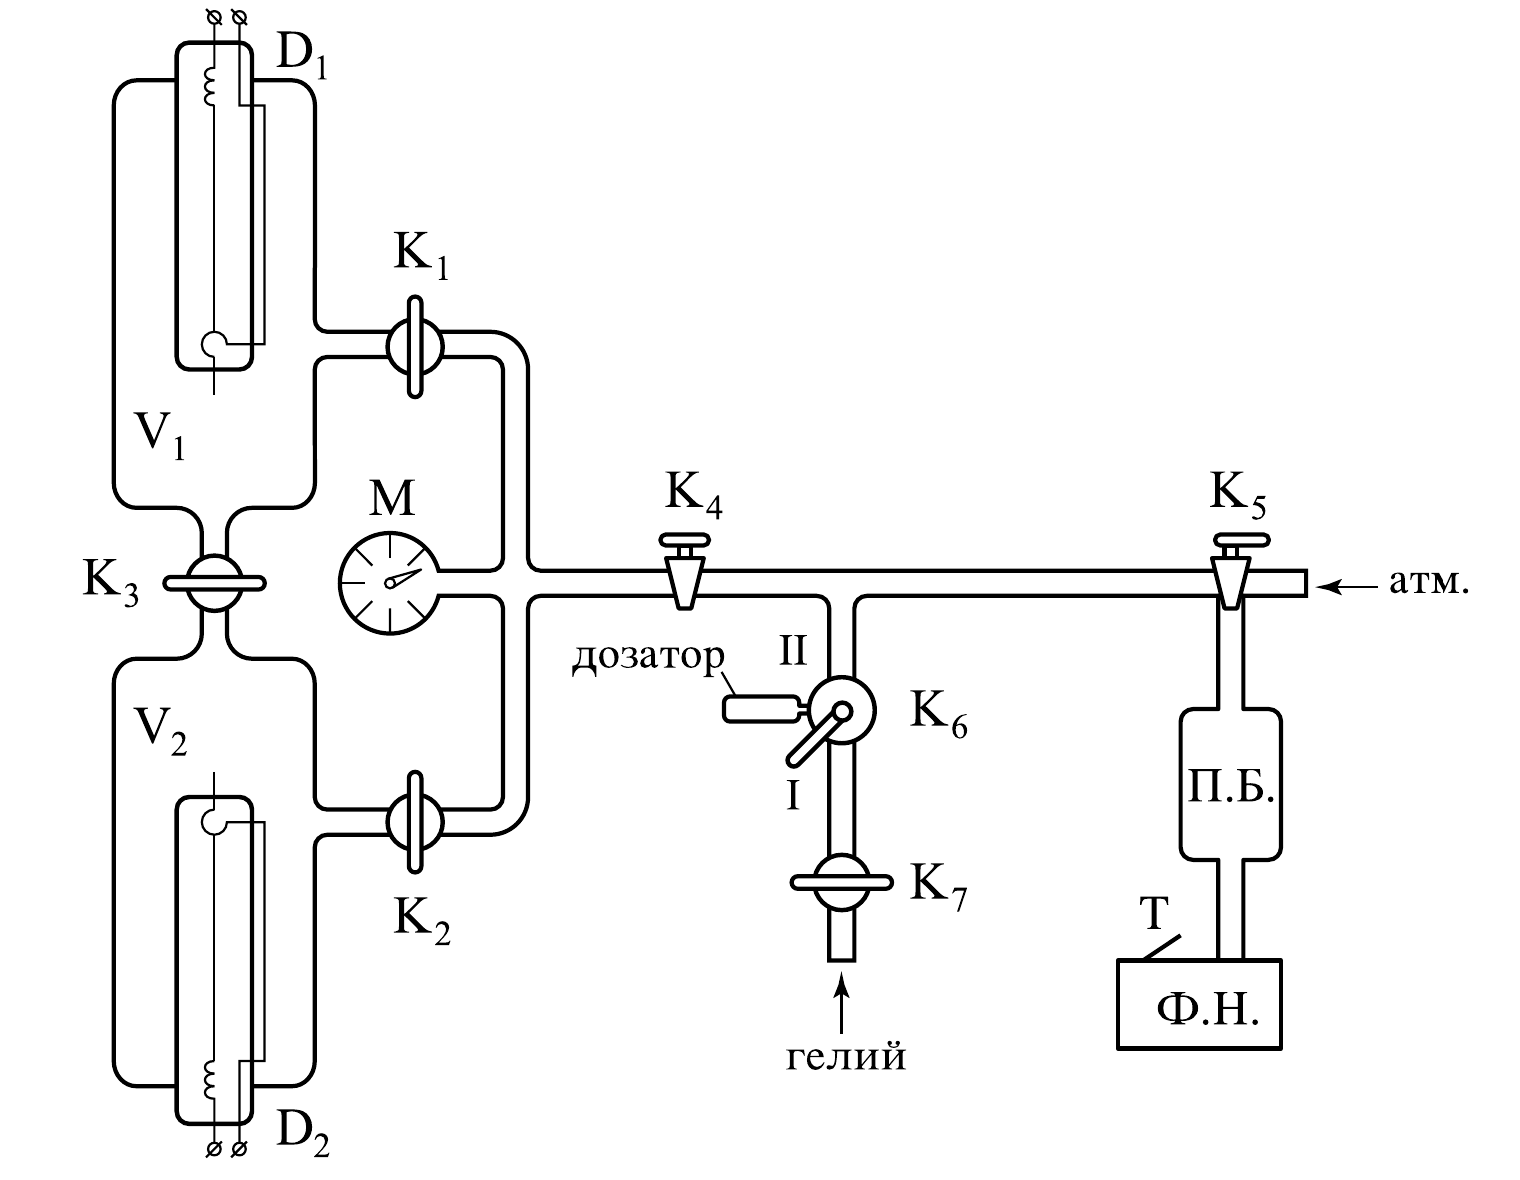
\includegraphics[scale = 0.273]{scheme1.png}
  \caption{Схема экспериментальной установки.}
\end{wrapfigure}
\end{document}
